% =====================================================================
% Medi-Script-AI: A Hybrid Detect--Read--Verify Pipeline for Digitising
% Handwritten Medical Prescriptions into Structured Records
% Build:  cd paper && latexmk -pdf main.tex
% =====================================================================
\documentclass[journal]{IEEEtran}

\usepackage[utf8]{inputenc}
\usepackage[T1]{fontenc}
\usepackage{amsmath,amssymb}
\usepackage{graphicx}
\usepackage{booktabs}
\usepackage{array}
\usepackage{multirow}
\usepackage{subcaption}
\usepackage{tikz}
\usepackage{xcolor}
\usepackage{listings}
\usepackage{algorithm}
\usepackage{algpseudocode}
\usepackage{cite}
\usepackage[hidelinks]{hyperref}
\usepackage{microtype}

% Shared TikZ styles for all Medi-Script-AI diagrams.
\usetikzlibrary{positioning,arrows.meta,fit,backgrounds,calc,shapes.geometric,decorations.pathreplacing}

\definecolor{cIn}{RGB}{90,90,90}
\definecolor{cDet}{RGB}{31,119,180}
\definecolor{cEnh}{RGB}{148,103,189}
\definecolor{cRec}{RGB}{214,39,40}
\definecolor{cPost}{RGB}{44,160,44}
\definecolor{cPar}{RGB}{255,127,14}
\definecolor{cLlm}{RGB}{23,190,207}
\definecolor{cOut}{RGB}{50,50,50}

\tikzset{
  base/.style={draw, rounded corners=2.5pt, align=center, font=\scriptsize,
               inner sep=3.5pt, minimum height=9mm, text width=2.35cm, line width=0.5pt},
  io/.style={base, fill=cIn!10, draw=cIn!80!black},
  det/.style={base, fill=cDet!12, draw=cDet!80!black},
  enh/.style={base, fill=cEnh!12, draw=cEnh!80!black},
  rec/.style={base, fill=cRec!10, draw=cRec!80!black},
  vpost/.style={base, fill=cPost!12, draw=cPost!80!black},
  par/.style={base, fill=cPar!14, draw=cPar!80!black},
  llm/.style={base, fill=cLlm!14, draw=cLlm!80!black},
  vout/.style={base, fill=cOut!10, draw=cOut, very thick},
  dec/.style={diamond, aspect=2.2, draw=cOut!80, fill=yellow!12, align=center,
              font=\scriptsize, inner sep=1pt, line width=0.5pt},
  small/.style={base, text width=1.45cm, minimum height=8mm, inner sep=2pt},
  arr/.style={-{Stealth[length=2.2mm]}, line width=0.6pt, draw=black!75},
  darr/.style={-{Stealth[length=2.2mm]}, line width=0.6pt, draw=black!60, dashed},
  lab/.style={font=\tiny\itshape, text=black!70, inner sep=1pt},
  lane/.style={draw=black!35, dashed, rounded corners=4pt, inner sep=6pt},
  lanelabel/.style={font=\scriptsize\bfseries, text=black!65},
}


\definecolor{codebg}{RGB}{245,246,248}
\lstdefinestyle{rec}{backgroundcolor=\color{codebg},basicstyle=\ttfamily\scriptsize,breaklines=true,
  frame=single,rulecolor=\color{black!20},columns=flexible,xleftmargin=2pt,xrightmargin=2pt}
\lstset{style=rec}

\newcommand{\sys}{\textsc{Medi-Script-AI}}
\hyphenation{pre-scrip-tion hand-writ-ten}

\begin{document}

\title{\sys: A Hybrid Detect--Read--Verify Pipeline for Digitising Handwritten Medical Prescriptions into Structured Records}

% TODO(authors): add institution name and e-mail addresses before submission.
\author{Mahakisore~M (CB.SC.U4AIE24333) and Yashwanth~B (CB.SC.U4AIE24360)\\
\textit{Department of Computer Science and Engineering (Artificial Intelligence)}\\
Course project, Deep Learning (22AIE304)}

\markboth{Medi-Script-AI: Technical Report}{Mahakisore and Yashwanth: Medi-Script-AI}
\maketitle

% ---------------------------------------------------------------------
\begin{abstract}
Handwritten prescriptions remain a leading source of dispensing errors, yet existing digitisation systems either classify isolated characters, rely on large proprietary corpora, or treat the page as a single OCR problem. We present \sys, a modular pipeline that separates \emph{where} information is written from \emph{what} it says and then \emph{verifies} the answer against medical knowledge. A fine-tuned YOLOv8-nano detector localises handwritten medicine lines; each line is enhanced and read by a three-tier recogniser (a multimodal vision-language model, falling back to a fine-tuned TrOCR-Large whose $N$-best list is rescored by a character-level domain language model); the text is corrected against a 384{,}604-entry medicine lexicon with TF-IDF character $n$-gram retrieval; and all remaining printed or demographic text is recovered with full-page EasyOCR, regular expressions and a spatial anchor parser. A constrained LLM stage re-assigns unclassified fragments and expands dosage abbreviations into patient-readable instructions. The detector reaches \textbf{86.1\% mAP50} (46.2\% mAP50--95, 81.9\% precision, 80.6\% recall) on a real handwritten-prescription benchmark, trains in about four minutes on one GPU and occupies 6.2\,MB. Qualitative error analysis of an earlier confidence-gated configuration shows \emph{safe failure}---an empty field rather than a fluent wrong drug---when recognition is uncertain, and also exposes the fluent-hallucination mode that motivates verification. We position the work against the recent CNN--MLP framework of Biswas \emph{et al.}~\cite{biswas2026novel}, enumerate which design limitations it removes, and state candidly which accuracy claims we cannot yet make.
\end{abstract}

\begin{IEEEkeywords}
handwritten text recognition, medical prescription digitisation, YOLOv8, TrOCR, vision-language models, lexicon correction, electronic health records
\end{IEEEkeywords}

% =====================================================================
\section{Introduction}\label{sec:intro}
\IEEEPARstart{M}{edical} prescriptions are the interface between a clinician's decision and the dispensed treatment. In much of South Asia they are still written by hand on pre-printed pads with irregular layouts, and illegible drug names or dosages are a recognised cause of preventable harm: the Institute of Medicine estimated that medication errors injure at least 1.5 million people per year in the United States, with the extra cost of drug-related injuries in hospitals alone at least \$3.5 billion annually~\cite{iom2007medicationerrors}. Manual transcription by pharmacists or data-entry staff is slow, error-prone and a barrier to electronic health record (EHR) integration.

A prescription is not an ordinary document. It is a \emph{semantically structured} artefact: different regions carry different kinds of information (patient demographics, diagnosis, one medicine per line with dosage), the printed header is machine-readable while the body is free-form handwriting, and the vocabulary---thousands of brand names, many absent from general language models---is highly specialised. Any practical system must therefore answer two questions in sequence: \emph{where} is each piece of information, and \emph{what} does it say?

\subsection{Problem statement}
Given one RGB photograph $P$ of a handwritten prescription, produce a structured record
\begin{equation}
\begin{split}
R&=\mathcal{F}(P)=\bigl(\text{doctor},\;\text{clinic},\;\text{date},\\
&\quad\text{patient}\!=\!(\text{name},\text{age},\text{sex}),\;\mathcal{M},\;\text{other}\bigr),
\end{split}
\label{eq:problem}
\end{equation}
where $\mathcal{M}=\{m_1,\dots,m_k\}$ is the ordered list of prescribed medicine lines (name, strength and dosage notation such as \texttt{1-0-1}). The system must prefer an \emph{abstention} (empty or flagged field) over a confidently wrong value, because in this domain a fluent error is more dangerous than an obvious omission.

\subsection{Motivation from the base study}
The study of Biswas \emph{et al.}~\cite{biswas2026novel} (hereafter the \emph{base paper}) is a comprehensive recent attempt at this task. It segments scanned prescriptions with contours, separates printed from handwritten patches with a CNN--SVM, and recognises each attribute (name, age, gender, symptom, medicine) with a CNN feature extractor followed by a multilayer perceptron trained on a very large private collection, exporting the result as CSV for EHR use. Its strengths are scale and an explicit end-to-end data path. Its design, however, has four limitations that motivated our work: (i)~recognition is \emph{closed-vocabulary classification of glyph or word classes} trained per attribute, so a drug name unseen at training time cannot be produced; (ii)~there is no explicit knowledge-based verification of drug names; (iii)~dosage notation and layout-dependent fields are not modelled; and (iv)~its reported figures depend on a proprietary data set that cannot be re-used or inspected. \sys{} is designed to address exactly these four points.

\subsection{Contributions}
\begin{enumerate}
  \item A \textbf{detect--read--verify architecture} that pairs a lightweight object detector with line-level sequence recognition instead of per-attribute glyph classifiers (Section~\ref{sec:method}).
  \item A \textbf{tiered recogniser}: multimodal LLM $\rightarrow$ fine-tuned TrOCR-Large with domain-LM rescoring $\rightarrow$ optional confidence-gated abstention, which keeps the system usable offline and exposes (rather than hides) hallucination.
  \item A \textbf{large-lexicon correction layer} using TF-IDF character $n$-gram retrieval (one sparse matrix--vector product over a 384{,}604-entry medicine list per query), with dosage-aware tokenisation.
  \item A \textbf{layout-aware parser} combining regular expressions with spatial anchor search for printed and demographic fields, including explicit fall-backs for common OCR confusions.
  \item A \textbf{constrained LLM post-processing stage} that fills only empty fields and translates dosage abbreviations without giving medical advice.
  \item An \textbf{incremental TrOCR training recipe} (v1$\rightarrow$v4) with synthetic dosage data, and an open, reproducible code base (Section~\ref{sec:impl}).
  \item A \textbf{candid evaluation} that reports the measured detector metrics, documents failure modes, and separates claims we can support from those we cannot (Section~\ref{sec:results}).
\end{enumerate}

% =====================================================================
\section{Related Work}\label{sec:related}

\subsection{Classical and classifier-based prescription recognition}
Early systems relied on fixed templates or keyword spotting with hidden Markov models over printed sections, and later on handcrafted features with SVM or naive-Bayes classifiers. The base paper~\cite{biswas2026novel} summarises this line and its limits: dependence on printed text, poor scalability and single-language scope. Digit and glyph recognisers trained on MNIST/EMNIST~\cite{cohen2017emnist} give strong isolated-character accuracy but need an explicit segmentation of characters, which cursive medical handwriting makes unreliable.

\subsection{CNN--MLP and CTC pipelines}
Convolutional feature extractors followed by recurrent layers and connectionist temporal classification (CTC)~\cite{graves2006ctc,shi2017crnn} are the standard recipe for line-level handwriting recognition. The base paper positions its model in this family but, in practice, uses CNN features with MLP classifiers over character and word classes. Classification heads bound the output space by construction, whereas sequence decoders can emit any string.

\subsection{Transformer-based recognition}
TrOCR~\cite{li2023trocr} replaces the CNN/RNN stack with an image Transformer encoder~\cite{dosovitskiy2021vit} and an autoregressive text Transformer decoder~\cite{vaswani2017attention}, pre-trained on large synthetic and real text-line corpora. It reads a whole line without character segmentation, but its decoder carries a general-language prior and can hallucinate fluent but unrelated words on illegible handwriting---a failure we observe directly (Section~\ref{sec:results}). OCR-free document transformers such as Donut~\cite{kim2022donut} and layout-aware models such as LayoutLMv3~\cite{huang2022layoutlmv3} treat the page holistically; in our test they transferred poorly from synthetic to real prescriptions.

\subsection{Detection-then-recognition}
Object detectors~\cite{redmon2016yolo,jocher2023yolov8} localise regions that are then passed to a recogniser. This decomposition lets each model be trained on the data it needs and exposes a clean place to insert domain knowledge between stages; it is the basis of \sys.

\subsection{Multimodal foundation models}
Large vision-language models~\cite{gemini2023} read handwriting zero-shot and can follow format instructions, but are remote services, rate-limited and opaque. We use one as the \emph{primary} reader while retaining a local fine-tuned model as fall-back, and constrain its prompts to transcription and abbreviation expansion.

\subsection{Gap}
Prior work either classifies glyphs/words inside a closed vocabulary, or applies one generic reader to the whole page. None combines (a) a learned line detector, (b) open-vocabulary sequence recognition, (c) large-lexicon verification with abstention, and (d) layout-aware parsing of the non-handwritten fields in one reproducible, offline-capable system. Table~\ref{tab:compare} makes this comparison explicit.

\begin{table*}[t]
\centering
\caption{Design-level comparison with the base study. Reported accuracies of the two systems are \emph{not} comparable (different data, private vs.\ public), and are therefore listed separately in Table~\ref{tab:baseacc}.}
\label{tab:compare}
\renewcommand{\arraystretch}{1.12}
\begin{tabular}{p{2.4cm}p{5.1cm}p{6.6cm}}
\toprule
\textbf{Aspect} & \textbf{Base paper~\cite{biswas2026novel}} & \textbf{\sys{} (this work)} \\
\midrule
Localisation & Contour detection + CNN--SVM printed/handwritten classifier & YOLOv8-nano learned line detector (6.2\,MB); EasyOCR + rules for printed text \\
Recognition unit & Characters / words classified per attribute (CNN features + MLP) & Whole line via image-to-text Transformer (TrOCR-Large) or multimodal LLM \\
Vocabulary & Closed (trained classes; EMNIST 47 classes) & Open decoding, constrained afterwards by a 384{,}604-entry lexicon \\
Knowledge verification & None reported & TF-IDF char $n$-gram lexicon correction; domain LM rescoring; abstention gate \\
Dosage notation & Not modelled & Synthetic-data fine-tuning (v4) and dosage-aware tokenisation \\
Printed text & Tesseract~\cite{smith2007tesseract} & EasyOCR (CRAFT + CRNN)~\cite{baek2019craft,jaidedai2020easyocr} \\
Layout fields (name, age, sex, date) & Separate per-attribute models on pre-cropped fields & Spatial anchor parser with regex fall-backs; works on free layouts \\
Post-processing & CSV export & LLM field re-assignment + dosage explanation; JSON / CSV \\
Training data & $>$400{,}000 proprietary prescriptions & 357-image public detection set, synthetic and pseudo-labelled crops (data and code released) \\
Failure behaviour & Wrong class label & Empty field in the gated configuration; verification flags otherwise \\
Deployment & Notebook & FastAPI service, web UI, Docker image, CLI \\
\bottomrule
\end{tabular}
\end{table*}

% =====================================================================
\section{Materials}\label{sec:data}

\subsection{Detection data}
We use two public Roboflow Universe exports of handwritten prescriptions with bounding boxes around handwritten medicine lines (Table~\ref{tab:data}). Dataset~D2 is the Bannari Amman Institute handwritten-recognition set~\cite{bannari2023handwritten}, on which the detector reported in Section~\ref{sec:results} was trained and evaluated; Dataset~D1 is a larger Roboflow export of doctors' prescriptions used for pipeline development. Roboflow exports include augmented copies of source images (visible as duplicate image names with different hash suffixes), so image counts overstate the number of independent prescriptions.

\begin{table}[t]
\centering
\caption{Detection data sets (single class: handwritten prescription line).}
\label{tab:data}
\begin{tabular}{lrrrr}
\toprule
 & \textbf{Train} & \textbf{Valid} & \textbf{Test} & \textbf{Total} \\
\midrule
D1 images & 884 & 219 & 135 & 1{,}238 \\
D1 boxes  & 3{,}976 & 972 & 556 & 5{,}504 \\
D2 images (Bannari) & 250 & 73 & 34 & 357 \\
D2 boxes & 740 & 216 & 90 & 1{,}046 \\
\bottomrule
\end{tabular}
\end{table}

\subsection{Recognition data}
\emph{Pseudo-labelled crops.} YOLO crops of real prescriptions were transcribed with a multimodal LLM prompted to output exactly what is written, including abbreviations and dosage symbols, producing an image/\texttt{Text} table used for TrOCR v2 and v3. \emph{Synthetic words.} For every entry of the lexicon, three renderings with random handwriting-style fonts (six cursive Google Fonts), colour, rotation and blur were generated at height 64\,px (3{,}531 training images in the released manifest). \emph{Synthetic dosage strings.} One thousand images of strings such as \texttt{1-0-1 x 5 days} or \texttt{1/2 - 0 - 1/2 for 1 week} were rendered the same way for the v4 increment. \emph{RxHandBD.} A public set of Bangladeshi prescription word images was used for an initial frozen-encoder run.

\subsection{Lexicons}
The medicine lexicon holds 384{,}604 Indian brand names; a symptom lexicon holds 35 phrases. A curated 1{,}142-entry subset was used in the earliest experiments (Section~\ref{sec:results}). The full medicine list is not redistributed (size and licence); the repository documents how to rebuild it.

\subsection{Ethics and privacy}
No data collected from patients are used. The data sets are public and de-identified at source. Because the LLM tier transmits crops to an external service, deployments handling real patient data should use the local-only configuration (Section~\ref{sec:impl}).

% =====================================================================
\section{Proposed Methodology}\label{sec:method}
Figure~\ref{fig:arch} gives the system overview and Fig.~\ref{fig:flow} the control flow of one inference. The pipeline has five stages organised into two parallel paths that are merged at the end.

\begin{figure*}[t]
\centering
\resizebox{\textwidth}{!}{% Figure: overall system architecture (two parallel paths merged by the LLM stage).
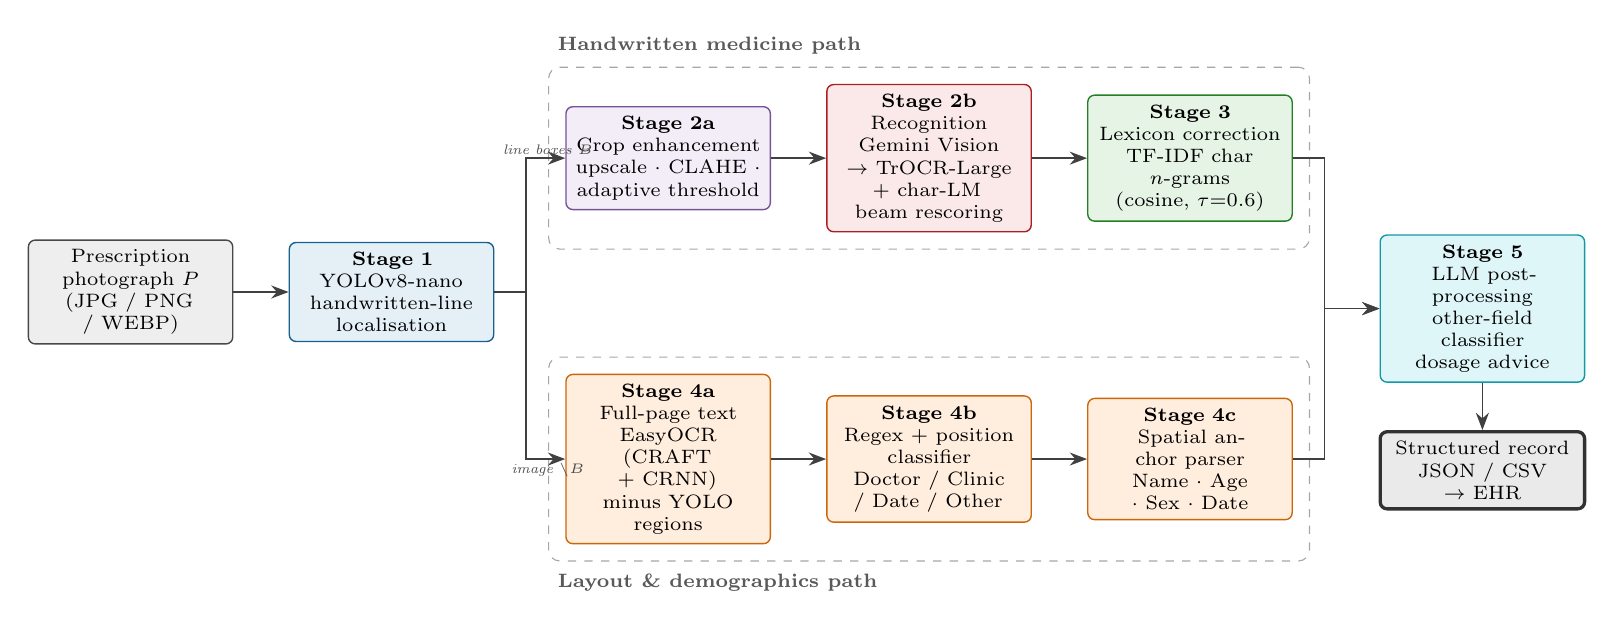
\begin{tikzpicture}[node distance=5mm and 7mm]
  % Input and Stage 1
  \node[io]  (in)  {Prescription photograph $P$\\ (JPG / PNG / WEBP)};
  \node[det, right=of in] (yolo) {\textbf{Stage 1}\\ YOLOv8-nano\\ handwritten-line localisation};

  % Handwritten medicine path (upper lane)
  \node[enh, above right=4mm and 9mm of yolo] (enh) {\textbf{Stage 2a}\\ Crop enhancement\\ upscale $\cdot$ CLAHE $\cdot$ adaptive threshold};
  \node[rec, right=of enh] (rec) {\textbf{Stage 2b}\\ Recognition\\ Gemini Vision $\rightarrow$ TrOCR-Large\\ + char-LM beam rescoring};
  \node[vpost, right=of rec] (lex) {\textbf{Stage 3}\\ Lexicon correction\\ TF-IDF char $n$-grams\\ (cosine, $\tau{=}0.6$)};

  % Layout / demographics path (lower lane)
  \node[par, below right=4mm and 9mm of yolo] (ocr) {\textbf{Stage 4a}\\ Full-page text\\ EasyOCR (CRAFT + CRNN)\\ minus YOLO regions};
  \node[par, right=of ocr] (cls) {\textbf{Stage 4b}\\ Regex + position\\ classifier\\ Doctor / Clinic / Date / Other};
  \node[par, right=of cls] (sp) {\textbf{Stage 4c}\\ Spatial anchor parser\\ Name $\cdot$ Age $\cdot$ Sex $\cdot$ Date};

  % Merge
  \coordinate (mid) at ($(lex.east)!0.5!(sp.east)$);
  \node[llm, anchor=west] (llm) at ($(mid)+(11mm,0)$) {\textbf{Stage 5}\\ LLM post-processing\\ other-field classifier\\ dosage advice};
  \node[vout, below=6mm of llm] (json) {Structured record\\ JSON / CSV $\rightarrow$ EHR};

  % Edges
  \draw[arr] (in) -- (yolo);
  \draw[arr] (yolo.east) -- ++(4mm,0) |- node[lab, pos=0.78, above] {line boxes $B$} (enh.west);
  \draw[arr] (yolo.east) -- ++(4mm,0) |- node[lab, pos=0.78, below] {image $\setminus B$} (ocr.west);
  \draw[arr] (enh) -- (rec);
  \draw[arr] (rec) -- (lex);
  \draw[arr] (ocr) -- (cls);
  \draw[arr] (cls) -- (sp);
  \draw[arr] (lex.east) -- ++(4mm,0) |- (llm.west);
  \draw[arr] (sp.east) -- ++(4mm,0) |- (llm.west);
  \draw[arr] (llm) -- (json);

  % Lanes
  \begin{scope}[on background layer]
    \node[lane, fit=(enh)(rec)(lex)] (laneU) {};
    \node[lane, fit=(ocr)(cls)(sp)] (laneL) {};
  \end{scope}
  \node[lanelabel, above=1pt of laneU.north west, anchor=south west] {Handwritten medicine path};
  \node[lanelabel, below=1pt of laneL.south west, anchor=north west] {Layout \& demographics path};
\end{tikzpicture}
}
\caption{\sys{} architecture. A learned detector (Stage~1) splits the image into handwritten medicine lines (upper path: enhancement, three-tier recognition, lexicon correction) and everything else (lower path: full-page OCR, regex/position classification, spatial anchor parsing). A constrained LLM stage merges both into the final structured record.}
\label{fig:arch}
\end{figure*}

\begin{figure*}[t]
\centering
\resizebox{\textwidth}{!}{% Figure: detailed methodology / control-flow of the inference procedure.
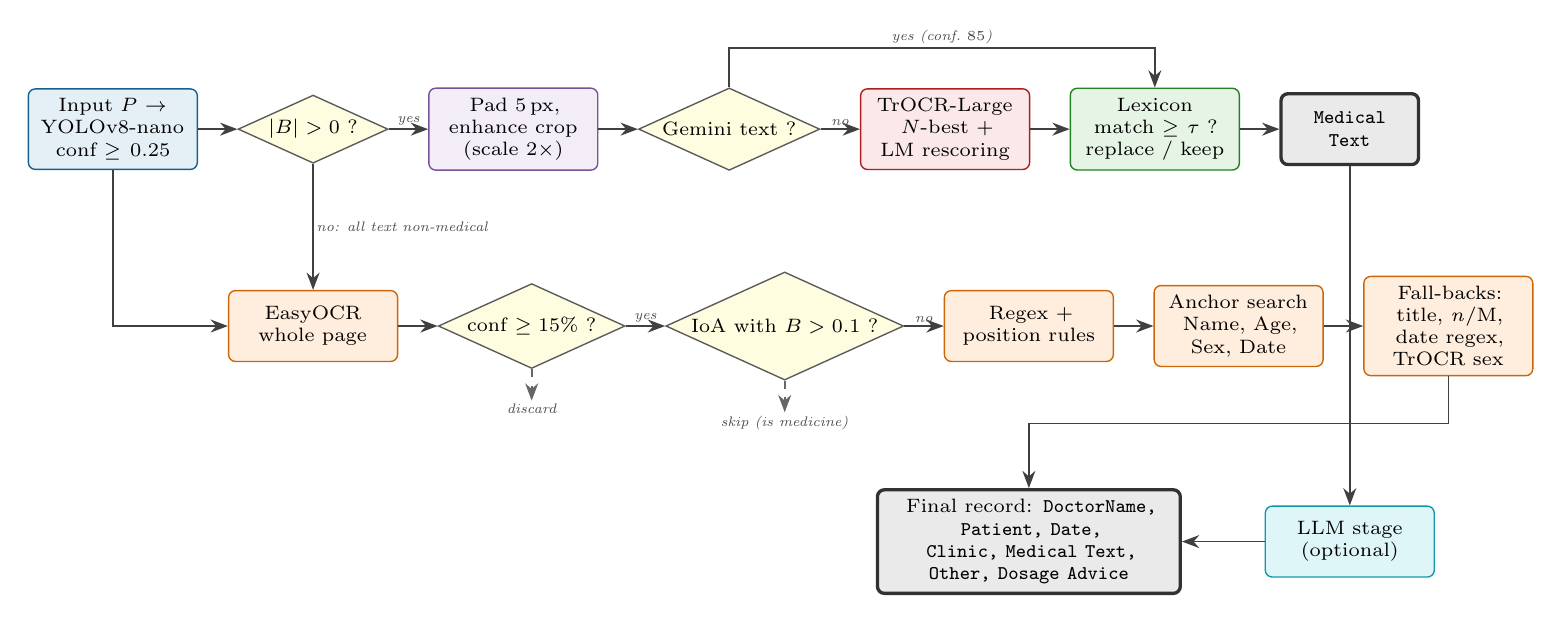
\begin{tikzpicture}[node distance=4mm and 5mm, base/.append style={text width=1.9cm}]
  % ---- Lane A: handwritten medicine lines ----
  \node[det] (a1) {Input $P$ $\rightarrow$ YOLOv8-nano\ conf $\ge 0.25$};
  \node[dec, right=of a1] (a2) {$|B|>0$ ?};
  \node[enh, right=of a2] (a3) {Pad 5\,px,\ enhance crop\ (scale $2\times$)};
  \node[dec, right=of a3] (a4) {Gemini\ text ?};
  \node[rec, right=of a4] (a5) {TrOCR-Large\ $N$-best $+$\ LM rescoring};
  \node[vpost, right=of a5] (a6) {Lexicon match\ $\ge\tau$ ?\ replace / keep};
  \node[vout, right=of a6, text width=1.5cm] (a7) {\texttt{Medical Text}};

  \draw[arr] (a1) -- (a2);
  \draw[arr] (a2) -- node[lab, above] {yes} (a3);
  \draw[arr] (a3) -- (a4);
  \draw[arr] (a4) -- node[lab, above] {no} (a5);
  \draw[arr] (a5) -- (a6);
  \draw[arr] (a6) -- (a7);
  \draw[arr] (a4.north) -- ++(0,5mm) -| node[lab, pos=0.25, above] {yes (conf.\ $85$)} (a6.north);

  % ---- Lane B: remaining text ----
  \node[par, below=16mm of a2] (b1) {EasyOCR\ whole page};
  \node[dec, right=of b1] (b2) {conf\ $\ge 15\%$ ?};
  \node[dec, right=of b2] (b3) {IoA with\ $B>0.1$ ?};
  \node[par, right=of b3] (b4) {Regex +\ position rules};
  \node[par, right=of b4] (b5) {Anchor search\ Name, Age,\ Sex, Date};
  \node[par, right=of b5] (b6) {Fall-backs:\ title, \textit{n}/M,\ date regex,\ TrOCR sex};

  \draw[arr] (a1.south) |- (b1.west);
  \draw[arr] (a2.south) -- node[lab, right] {no: all text non-medical} (b1.north);
  \draw[arr] (b1) -- (b2);
  \draw[arr] (b2) -- node[lab, above] {yes} (b3);
  \draw[arr] (b3) -- node[lab, above] {no} (b4);
  \draw[arr] (b4) -- (b5);
  \draw[arr] (b5) -- (b6);
  \draw[darr] (b2.south) -- ++(0,-4mm) node[lab, below] {discard};
  \draw[darr] (b3.south) -- ++(0,-4mm) node[lab, below] {skip (is medicine)};

  % ---- Merge ----
  \node[vout, below=16mm of b4, text width=3.6cm] (m) {Final record: \texttt{DoctorName, Patient, Date, Clinic, Medical Text, Other, Dosage Advice}};
  \node[llm] (l) at (a7 |- m) {LLM stage\\ (optional)};
  \draw[arr] (b6.south) -- ++(0,-6mm) -| (m.north);
  \draw[arr] (a7.south) -- (l.north);
  \draw[arr] (l.west) -- (m.east);
\end{tikzpicture}
}
\caption{Control flow of a single inference. Diamonds are decisions; dashed arrows denote discarded or skipped items. The Gemini branch is optional: without an API key every crop takes the local TrOCR route.}
\label{fig:flow}
\end{figure*}

\begin{figure*}[t]
\centering
\resizebox{!}{0.40\textheight}{% Figure: pipeline of the base paper (Biswas et al.) versus Medi-Script-AI.
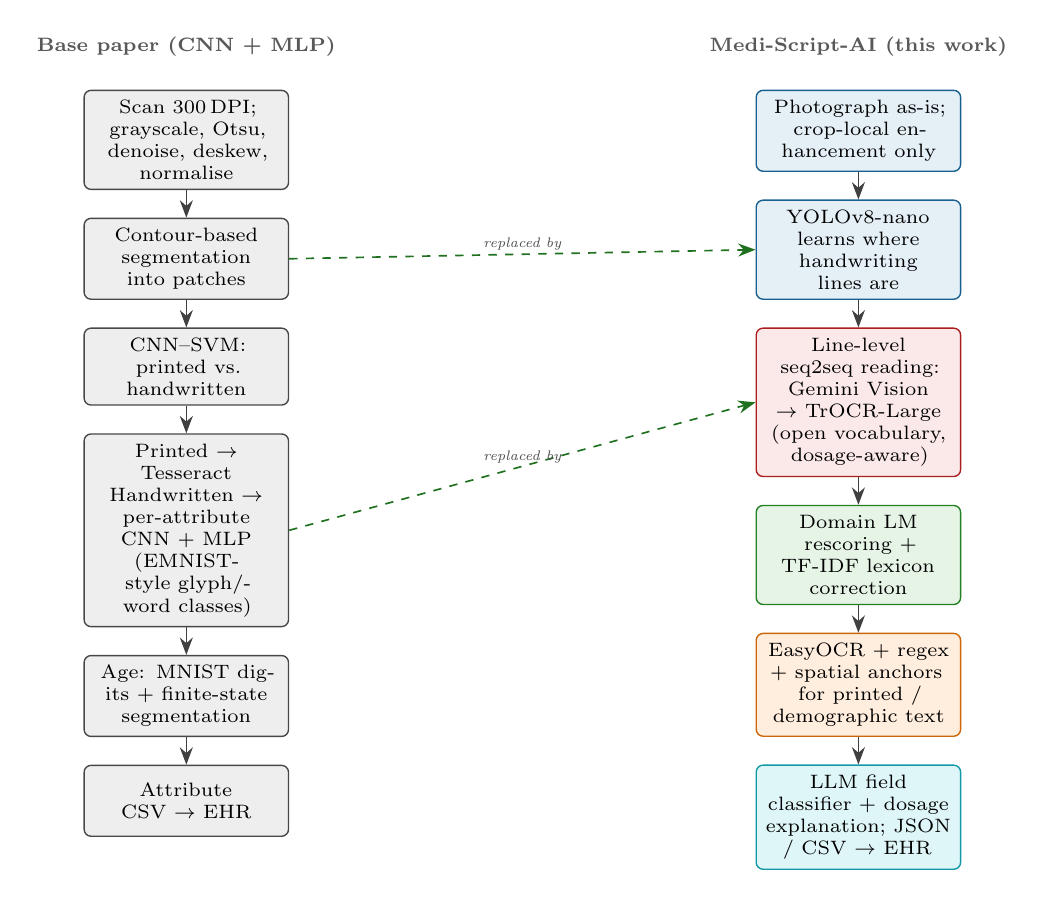
\begin{tikzpicture}[node distance=3.5mm, font=\scriptsize]
  \tikzset{col/.style={base, text width=3.5cm, minimum height=7.5mm}}
  % left column: base paper
  \node[lanelabel] (hl) {Base paper (CNN + MLP)};
  \node[col, io, below=3mm of hl] (l1) {Scan 300\,DPI; grayscale, Otsu,\\ denoise, deskew, normalise};
  \node[col, io, below=of l1] (l2) {Contour-based segmentation\\ into patches};
  \node[col, io, below=of l2] (l3) {CNN--SVM: printed vs.\ handwritten};
  \node[col, io, below=of l3] (l4) {Printed $\rightarrow$ Tesseract\\ Handwritten $\rightarrow$ per-attribute\\ CNN + MLP (EMNIST-style glyph/word classes)};
  \node[col, io, below=of l4] (l5) {Age: MNIST digits + finite-state\\ segmentation};
  \node[col, io, below=of l5] (l6) {Attribute CSV $\rightarrow$ EHR};
  \foreach \a/\b in {l1/l2,l2/l3,l3/l4,l4/l5,l5/l6} \draw[arr] (\a) -- (\b);

  % right column: ours
  \node[lanelabel, right=45mm of hl] (hr) {Medi-Script-AI (this work)};
  \node[col, det, below=3mm of hr] (r1) {Photograph as-is;\\ crop-local enhancement only};
  \node[col, det, below=of r1] (r2) {YOLOv8-nano learns where\\ handwriting lines are};
  \node[col, rec, below=of r2] (r3) {Line-level seq2seq reading:\\ Gemini Vision $\rightarrow$ TrOCR-Large\\ (open vocabulary, dosage-aware)};
  \node[col, vpost, below=of r3] (r4) {Domain LM rescoring $+$\\ TF-IDF lexicon correction};
  \node[col, par, below=of r4] (r5) {EasyOCR + regex + spatial anchors\\ for printed / demographic text};
  \node[col, llm, below=of r5] (r6) {LLM field classifier $+$ dosage\\ explanation; JSON / CSV $\rightarrow$ EHR};
  \foreach \a/\b in {r1/r2,r2/r3,r3/r4,r4/r5,r5/r6} \draw[arr] (\a) -- (\b);

  % correspondences
  \draw[darr, cPost!70!black] (l2.east) -- node[lab, above, pos=0.5] {replaced by} (r2.west);
  \draw[darr, cPost!70!black] (l4.east) -- node[lab, above, pos=0.5] {replaced by} (r3.west);
\end{tikzpicture}
}
\caption{Side-by-side pipelines: the base paper's CNN--MLP chain (left) and \sys{} (right). Dashed arrows indicate which base-paper component each of our stages replaces.}
\label{fig:compare}
\end{figure*}

\subsection{Stage 1: handwritten-line localisation}
We fine-tune \textbf{YOLOv8-nano}~\cite{jocher2023yolov8} (3.0\,M parameters, 8.1\,GFLOPs) as a single-class detector at $640{\times}640$ input. Detections with confidence $\ge 0.25$ form the set $B=\{b_j\}$ of line boxes. The nano variant was chosen because it trains in minutes, produces a 6.2\,MB checkpoint small enough to ship in the repository, and runs in milliseconds, which leaves the latency budget to the recognisers. Each box is padded by 5\,px before cropping to avoid clipping ascenders and descenders of cursive strokes.

\subsection{Stage 2a: crop enhancement}\label{sec:enhance}
Handwritten crops are small, low-contrast and unevenly lit. Each crop $C$ passes through the chain in Fig.~\ref{fig:enhance}: Lanczos upscaling by $s{=}2$, grayscale conversion $I_{\text{gray}}=0.299R+0.587G+0.114B$, a $3{\times}3$ Gaussian blur, contrast-limited adaptive histogram equalisation (CLAHE)~\cite{zuiderveld1994clahe} with clip limit 2.5 on a $4{\times}4$ grid, adaptive Gaussian thresholding (block 15, constant 8), and a $2{\times}2$ dilation that reconnects thin strokes. Local rather than global thresholding is deliberate: global Otsu binarisation~\cite{otsu1979threshold}, used on the full page by the base paper, fails under uneven illumination, and a per-crop operation adapts to each line's lighting. A non-local-means denoiser was replaced by the Gaussian blur because it was $O(N^2)$ and stalled on large crops, while the blur costs under one millisecond.

\begin{figure*}[t]
\centering
\resizebox{0.95\textwidth}{!}{% Figure: crop-enhancement chain applied to every YOLO crop.
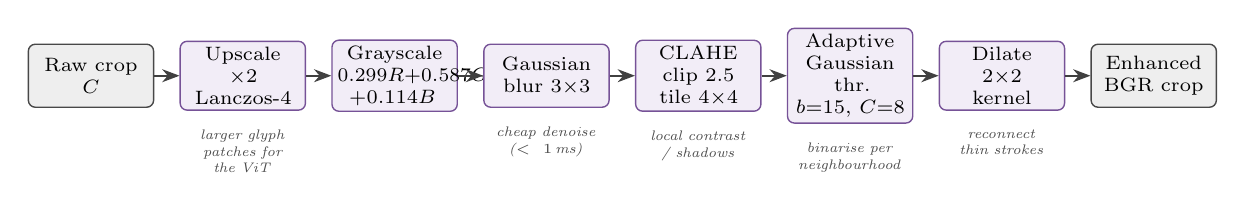
\begin{tikzpicture}[node distance=3.2mm]
  \node[io, small] (c0) {Raw crop\\ $C$};
  \node[enh, small, right=of c0] (c1) {Upscale\\ $\times 2$\\ Lanczos-4};
  \node[enh, small, right=of c1] (c2) {Grayscale\\ $0.299R{+}0.587G$\\ $+0.114B$};
  \node[enh, small, right=of c2] (c3) {Gaussian\\ blur $3{\times}3$};
  \node[enh, small, right=of c3] (c4) {CLAHE\\ clip $2.5$\\ tile $4{\times}4$};
  \node[enh, small, right=of c4] (c5) {Adaptive\\ Gaussian\\ thr.\ $b{=}15,\,C{=}8$};
  \node[enh, small, right=of c5] (c6) {Dilate\\ $2{\times}2$\\ kernel};
  \node[io, small, right=of c6] (c7) {Enhanced\\ BGR crop};
  \foreach \a/\b in {c0/c1,c1/c2,c2/c3,c3/c4,c4/c5,c5/c6,c6/c7} \draw[arr] (\a) -- (\b);
  \node[lab, below=2mm of c1, text width=1.6cm, align=center] {larger glyph patches for the ViT};
  \node[lab, below=2mm of c3, text width=1.9cm, align=center] {cheap denoise ($<1$\,ms)};
  \node[lab, below=2mm of c4, text width=1.9cm, align=center] {local contrast / shadows};
  \node[lab, below=2mm of c5, text width=2.1cm, align=center] {binarise per neighbourhood};
  \node[lab, below=2mm of c6, text width=1.8cm, align=center] {reconnect thin strokes};
\end{tikzpicture}
}
\caption{Crop-enhancement chain (Stage 2a). Parameters are those used in the released code.}
\label{fig:enhance}
\end{figure*}

\subsection{Stage 2b: three-tier recognition}\label{sec:recog}
\paragraph{Tier 1: multimodal LLM.} The enhanced crop is sent to a Gemini vision model~\cite{gemini2023} with a prompt that casts it as a pharmacist reading \emph{one} medicine line, forbids explanations, and requires the literal token \texttt{UNREADABLE} when the line is unclear or not a medicine. An \texttt{UNREADABLE} reply or any API error returns the empty string and triggers Tier~2.

\paragraph{Tier 2: fine-tuned TrOCR-Large.} The crop is resized to $384{\times}384$ and split into $16{\times}16$ patches; an encoder $E$ produces visual tokens and an autoregressive decoder factorises
\begin{equation}
p(t\mid C)=\prod_{k=1}^{|t|}p\bigl(t_k\mid t_{<k},E(C)\bigr).
\end{equation}
Decoding uses beam search ($N{=}2$ returned hypotheses for medicine fields, \texttt{no\_repeat\_ngram\_size}$=3$, at most 24 new tokens). The confidence of hypothesis $t_i$ is the mean token probability, $c_i=100\cdot\frac{1}{|t_i|}\sum_k p(t_{i,k}\mid\cdot)$. The newest available checkpoint (v3, v2, v1; the v4 dosage checkpoint is opt-in) is loaded, and the public \texttt{trocr-large-handwritten} model is the last resort.

\paragraph{Domain language-model rescoring.} Because a general decoder prefers fluent English, hypotheses are re-ranked with a character trigram model trained on the lexicons ($|V|$ symbols, Laplace smoothing):
\begin{align}
\mathrm{LM}(t)&=\frac{1}{|t|}\sum_{j}\log\frac{n(g_j)+1}{n(\mathrm{ctx}_j)+|V|+1},\\
s_i&=\frac{c_i}{100}+0.5\,\mathrm{LM}(t_i)+\mathbb{1}\bigl[t_i\in\mathcal{L}\bigr],
\label{eq:rescore}
\end{align}
where $g_j$ is the $j$-th character trigram, $\mathrm{ctx}_j$ its two-character context, and $\mathcal{L}$ the lexicon. The hypothesis with the highest $s_i$ is kept; its original $c_i$ is returned as confidence.

\paragraph{Tier 3: abstention.} If neither reader yields text the field is empty. In the field-level configuration used for the case studies, a field whose fused confidence falls below the gate (Eq.~\ref{eq:conf}) is additionally dropped rather than guessed. The default page-level path currently keeps the uncorrected reading and does not yet apply this gate; porting it is listed as future work.

\begin{figure*}[t]
\centering
\resizebox{0.95\textwidth}{!}{% Figure: Stage 2b/3 internals: TrOCR decoding, LM rescoring, lexicon correction.
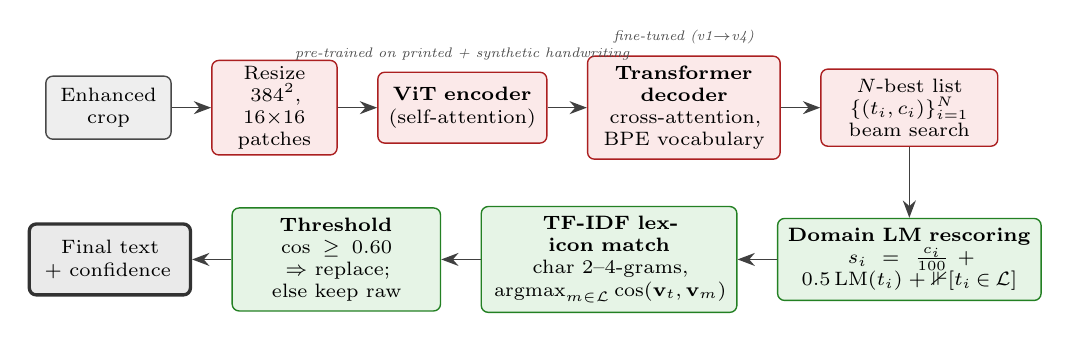
\begin{tikzpicture}[node distance=4mm and 5mm]
  \node[io, small] (x) {Enhanced\\ crop};
  \node[rec, small, right=of x] (patch) {Resize\\ $384^2$,\\ $16{\times}16$ patches};
  \node[rec, right=of patch, text width=1.9cm] (enc) {\textbf{ViT encoder}\\ (self-attention)};
  \node[rec, right=of enc, text width=2.2cm] (dec) {\textbf{Transformer decoder}\\ cross-attention,\\ BPE vocabulary};
  \node[rec, right=of dec, text width=2.0cm] (nb) {$N$-best list\\ $\{(t_i,c_i)\}_{i=1}^{N}$\\ beam search};

  \node[vpost, below=9mm of nb, text width=3.1cm] (lm) {\textbf{Domain LM rescoring}\\ $s_i = \frac{c_i}{100} + 0.5\,\mathrm{LM}(t_i) + \mathbb{1}[t_i\!\in\!\mathcal{L}]$};
  \node[vpost, left=of lm, text width=3.0cm] (tf) {\textbf{TF-IDF lexicon match}\\ char 2--4-grams,\\ $\operatorname{argmax}_{m\in\mathcal{L}}\cos(\mathbf v_t,\mathbf v_m)$};
  \node[vpost, left=of tf, text width=2.4cm] (th) {\textbf{Threshold}\\ $\cos\ge 0.60$ $\Rightarrow$ replace;\\ else keep raw};
  \node[vout, left=of th, text width=1.8cm] (res) {Final text\\ $+$ confidence};

  \draw[arr] (x) -- (patch);
  \draw[arr] (patch) -- (enc);
  \draw[arr] (enc) -- (dec);
  \draw[arr] (dec) -- (nb);
  \draw[arr] (nb) -- (lm);
  \draw[arr] (lm) -- (tf);
  \draw[arr] (tf) -- (th);
  \draw[arr] (th) -- (res);

  \node[lab, above=1mm of enc] {pre-trained on printed + synthetic handwriting};
  \node[lab, above=1mm of dec] {fine-tuned (v1$\rightarrow$v4)};
\end{tikzpicture}
}
\caption{Tier-2 recognition and Stage-3 verification: TrOCR $N$-best decoding, domain-LM rescoring (Eq.~\ref{eq:rescore}) and TF-IDF lexicon matching.}
\label{fig:recognition}
\end{figure*}

\subsection{Stage 3: lexicon correction}\label{sec:lexicon}
Exact fuzzy search over $\approx3.8{\times}10^{5}$ names with Levenshtein distance~\cite{levenshtein1966binary} is too slow per crop. We instead index the lexicon once with character-$n$-gram TF-IDF~\cite{salton1988tfidf} ($n\in[2,4]$, word-boundary padded) and retrieve the nearest entry by cosine similarity,
\begin{equation}
m^\star=\operatorname*{arg\,max}_{m\in\mathcal{L}}\;\frac{\mathbf v_q\cdot\mathbf v_m}{\lVert\mathbf v_q\rVert\,\lVert\mathbf v_m\rVert},
\end{equation}
which tolerates insertions, deletions and substitutions typical of OCR (e.g.\ \texttt{Amoxcilin}$\to$\texttt{Amoxicillin}). A medicine line such as \texttt{Tab. Ozad 100 BC 7 AM} contains non-drug tokens, so the line is first split at digits and dosage keywords (\texttt{tab, cap, syr, inj, bd, od, tds, sos, hs, ac, pc, mg, ml, \ldots}) into candidate word sequences. For each sequence the longest prefix whose best cosine is $\ge 0.60$ is substituted in place, leaving strengths and frequencies untouched. Text below threshold is returned unchanged, which is what allows the gate to expose genuinely unreadable lines instead of inventing a drug.

An RapidFuzz~\cite{bachmann2020rapidfuzz} \texttt{WRatio} matcher with a first-letter index is used for the small field lexicons (gender, symptoms), and a character trie (\texttt{LexiconTrie}) provides $O(k)$ exact and prefix look-ups for the LM and for the optional TrOCR/EasyOCR reconciliation module (agreement if $\mathrm{ratio}>85$).

\paragraph{Symbol-aware repairs.} Two regular rewrites address systematic confusions: \texttt{1H1}$\to$\texttt{1+1} (letter $H$ read for the plus sign) and \texttt{400mg16mg}$\to$\texttt{400mg/16mg} (dropped slash). The earlier unconditional substitution of $H,l,O\to +,1,0$ over the whole string corrupted drug names; the released version only rewrites tokens that look like dosage notation.

\paragraph{Confidence fusion.} The stage confidences---segmentation $c_{\text{seg}}$, recognition $c_{\text{rec}}$ and validation $c_{\text{val}}$ (90 if the lexicon changed the text, 55 if kept, 10 if no match)---are combined as
\begin{equation}
c=\min\!\Bigl(0.2\,c_{\text{seg}}+0.3\,c_{\text{rec}}+0.5\,c_{\text{val}},\;\; \min(c_{\text{seg}},c_{\text{rec}},c_{\text{val}})+15\Bigr),
\label{eq:conf}
\end{equation}
so that one very weak stage cannot be hidden by two strong ones. In the field-level configuration, fields with $c<15$, or a prescription field with $c_{\text{val}}<50$, are dropped.

\subsection{Stage 4: layout and demographic parsing}\label{sec:parse}
Everything outside the detected boxes is read by EasyOCR (CRAFT detector~\cite{baek2019craft} and CRNN recogniser~\cite{shi2017crnn,jaidedai2020easyocr}). Fragments with OCR confidence $<15\%$ are discarded, and a fragment $b$ is excluded when its intersection-over-area with any line box exceeds 0.1:
\begin{equation}
\mathrm{IoA}(b,B)=\max_{b_j\in B}\frac{|b\cap b_j|}{|b|}>0.1 .
\end{equation}
Remaining fragments are classified by ordered regular-expression rules plus position priors (Table~\ref{tab:rules}); normalised $(x_c,y_c)$ coordinates implement the observation that hospital information sits in the top and bottom bands or the left margin.

\begin{table}[t]
\centering
\caption{Ordered classification rules (first match wins).}
\label{tab:rules}
\small
\begin{tabular}{p{1.6cm}p{6.3cm}}
\toprule
\textbf{Class} & \textbf{Rule} \\
\midrule
DoctorName & \texttt{dr.}, \texttt{md}, \texttt{mbbs}, \texttt{prof.} \\
PatientInfo & \texttt{name/namc/age/sex/gender/patient}; or \texttt{\textbackslash d\{1,3\}\,/\,[mf]}, \texttt{\textbackslash d+\,yrs} \\
Date & \texttt{date}, or \texttt{dd/mm/yy}; or a 6--10 char digit string in the top-right quadrant \\
Hospital / Clinic & $y_c<0.25$ or $y_c>0.8$ or $x_c<0.25$, and keyword (\texttt{hospital, clinic, care, institute, \ldots}) or $\ge2$ words \\
Other & fall-through \\
\bottomrule
\end{tabular}
\end{table}

\paragraph{Spatial anchor parsing.} Labels such as \emph{Name}, \emph{Age}, \emph{Sex} and \emph{Date} act as anchors (matched exactly or by fuzzy ratio $\ge75$ to survive \texttt{Name}$\to$\texttt{Namc}). For an anchor $a$ the value is the nearest fragment $b$ to its right on the same line (Fig.~\ref{fig:spatial}),
\begin{equation}
b^\star=\operatorname*{arg\,min}_{b:\;|c_y(b)-c_y(a)|<\delta,\;x_1(b)\ge x_2(a)}\bigl(x_1(b)-x_2(a)\bigr),
\end{equation}
with $\delta=30$\,px (15 to join a multi-word name, which ends at the \emph{Sex} anchor; 45 for sex; 75 for date, where the best digit-and-separator candidate is preferred). Fall-backs recover from missing anchors: a title (\emph{Mr./Mrs./Mast.}) implies a name; the patterns \texttt{28/M} and \texttt{12\,yrs\,/\,F} yield age and sex; date patterns tolerate alphanumeric OCR errors; a misread \texttt{47/F} (``4\,yr/F'') is repaired; the \emph{Sex} value is re-read from a crop with TrOCR when EasyOCR fails; and \texttt{1717/24}$\to$\texttt{17/7/24} corrects a slash read as ``1''.

\begin{figure*}[t]
\centering
\resizebox{0.9\textwidth}{!}{% Figure: spatial anchor parsing on an abstract prescription layout (no real patient data).
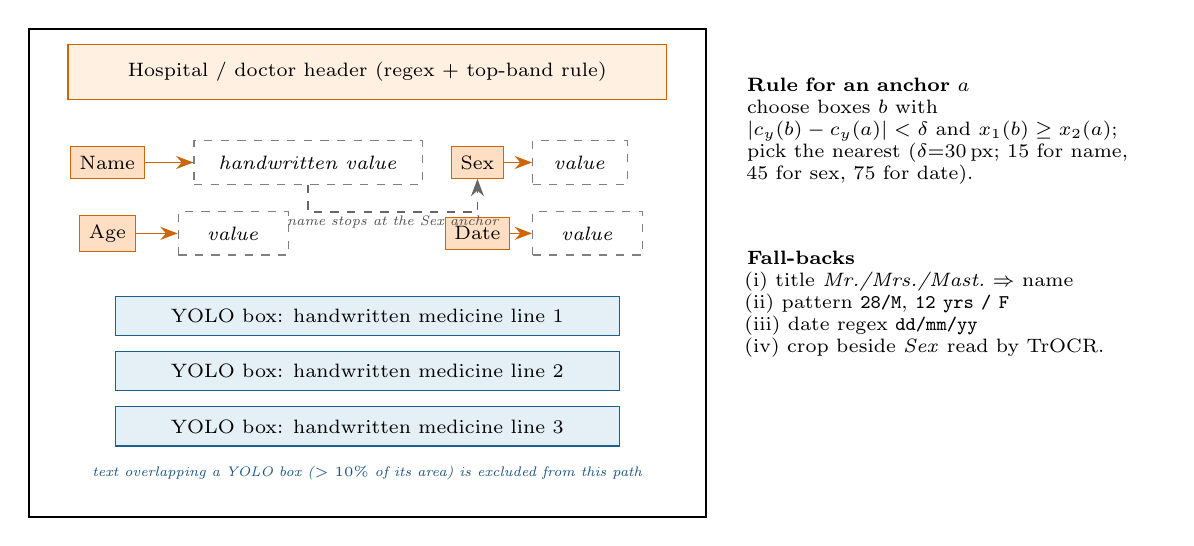
\begin{tikzpicture}[x=1cm,y=1cm, font=\scriptsize]
  % page
  \draw[line width=0.7pt, fill=white] (0,0) rectangle (8.6,6.2);
  % header (hospital / doctor)
  \node[draw=cPar!80!black, fill=cPar!12, minimum width=7.6cm, minimum height=0.7cm] at (4.3,5.65) {Hospital / doctor header (regex + top-band rule)};
  % anchor row 1
  \node[draw=cPar!80!black, fill=cPar!25] (nm) at (1.0,4.5) {Name};
  \node[draw=black!50, dashed, minimum width=2.9cm, minimum height=0.55cm] (nv) at (3.55,4.5) {\textit{handwritten value}};
  \node[draw=cPar!80!black, fill=cPar!25] (sx) at (5.7,4.5) {Sex};
  \node[draw=black!50, dashed, minimum width=1.2cm, minimum height=0.55cm] (sv) at (7.0,4.5) {\textit{value}};
  % anchor row 2
  \node[draw=cPar!80!black, fill=cPar!25] (ag) at (1.0,3.6) {Age};
  \node[draw=black!50, dashed, minimum width=1.4cm, minimum height=0.55cm] (av) at (2.6,3.6) {\textit{value}};
  \node[draw=cPar!80!black, fill=cPar!25] (dt) at (5.7,3.6) {Date};
  \node[draw=black!50, dashed, minimum width=1.4cm, minimum height=0.55cm] (dv) at (7.1,3.6) {\textit{value}};
  % YOLO medicine boxes
  \foreach \y/\t in {2.55/line 1, 1.85/line 2, 1.15/line 3} {
    \node[draw=cDet!80!black, fill=cDet!12, minimum width=6.4cm, minimum height=0.5cm] at (4.3,\y) {YOLO box: handwritten medicine \t};
  }
  \node[font=\tiny\itshape, text=cDet!70!black] at (4.3,0.55) {text overlapping a YOLO box ($>10\%$ of its area) is excluded from this path};

  % arrows
  \draw[arr, cPar!80!black] (nm.east) -- (nv.west);
  \draw[arr, cPar!80!black] (sx.east) -- (sv.west);
  \draw[arr, cPar!80!black] (ag.east) -- (av.west);
  \draw[arr, cPar!80!black] (dt.east) -- (dv.west);
  % stop condition
  \draw[darr] (nv.south) -- ++(0,-0.35) -| node[lab, pos=0.25, below] {name stops at the \textit{Sex} anchor} (sx.south);
  % legend
  \node[anchor=west, text width=5.2cm, align=left] at (9.0,4.9) {\textbf{Rule for an anchor $a$}\\ choose boxes $b$ with\\ $|c_y(b)-c_y(a)|<\delta$ and $x_1(b)\ge x_2(a)$;\\ pick the nearest ($\delta{=}30$\,px; $15$ for name,\\ $45$ for sex, $75$ for date).};
  \node[anchor=west, text width=5.2cm, align=left] at (9.0,2.7) {\textbf{Fall-backs}\\ (i) title \textit{Mr./Mrs./Mast.}\ $\Rightarrow$ name\\ (ii) pattern \texttt{28/M}, \texttt{12 yrs / F}\\ (iii) date regex \texttt{dd/mm/yy}\\ (iv) crop beside \textit{Sex} read by TrOCR.};
\end{tikzpicture}
}
\caption{Spatial anchor parsing on an abstract layout. Orange boxes are anchors found by EasyOCR; dashed boxes are the values located to their right. Blue boxes are YOLO regions handled by the other path.}
\label{fig:spatial}
\end{figure*}

\subsection{Stage 5: constrained LLM post-processing}\label{sec:llm}
Two optional calls use a Gemini text model. The \emph{other-field classifier} receives the residual \texttt{Other} string and returns JSON assigning fragments to patient name, age, sex, doctor, date or clinic; the result is applied \emph{only to fields that are still empty} (clinic text is appended), and leftovers stay in \texttt{Other}. A doctor name must carry an explicit title, otherwise it is a patient name. The \emph{dosage-advice generator} converts lines such as \texttt{T. Ambulax 1 BD} into ``Take 1 twice a day (BD)''. Both prompts forbid diagnosis or advice beyond translating abbreviations, and any API failure leaves the record unchanged.

\subsection{End-to-end procedure}
Algorithm~\ref{alg:infer} summarises inference.

\begin{algorithm}[t]
\caption{\sys{} inference}\label{alg:infer}
\begin{algorithmic}[1]
\Require image $P$; lexicon $\mathcal{L}$; thresholds $\theta_{\text{det}}{=}0.25$, $\tau{=}0.60$
\State $B\gets\textsc{Yolo}(P,\theta_{\text{det}})$; $\mathcal{M}\gets[\,]$
\For{$b\in B$}
  \State $C\gets\textsc{Enhance}(\textsc{Crop}(P,b,\mathrm{pad}{=}5))$
  \State $t\gets\textsc{Gemini}(C)$
  \If{$t=\varnothing$} $t\gets\textsc{Rescore}(\textsc{TrOcr}(C))$ \EndIf
  \State $t\gets\textsc{LexiconCorrect}(t,\mathcal{L},\tau)$; append $t$ to $\mathcal{M}$
\EndFor
\State $F\gets\textsc{EasyOcr}(P)$; drop low-confidence and $\mathrm{IoA}>0.1$ fragments
\State classify each $f\in F$ (Table~\ref{tab:rules}); run anchor parser $\Rightarrow$ patient, date
\State \textbf{optional:} $R\gets\textsc{OtherClassifier}(R)$; advice $\gets\textsc{Dosage}(\mathcal{M})$
\State \Return $R$
\end{algorithmic}
\end{algorithm}

% =====================================================================
\section{Training}\label{sec:train}

\subsection{Detector}
YOLOv8-nano was initialised from COCO weights and fine-tuned for 50 epochs at $640{\times}640$ on D2 (Tesla T4, about four minutes, 0.067 GPU-hours), with the library's default mosaic and colour augmentations and early stopping (patience 10 in the released training script). The checkpoint is stored at \texttt{models/yolo/yolo\_real\_world\_best.pt}.

\subsection{Recogniser lineage}
TrOCR-Large was adapted in four documented steps (Fig.~\ref{fig:training}, Table~\ref{tab:hyper}). The reasoning was to \emph{progressively unlock capacity while lowering the learning rate}: an initial run trains only the decoder so the encoder keeps its general stroke features; the cursive-specialisation run (v3) unfreezes the top four ViT layers, injects frequent drug names as single tokens (the embedding matrix is resized accordingly) to shorten decoding, and adds elastic and perspective distortion to emulate slant and stretch; the final increment (v4) teaches dosage syntax with synthetic data at a learning rate small enough to avoid catastrophic forgetting. Model selection uses the character error rate (CER) on a 15\% validation split with early stopping.

\begin{table*}[t]
\centering
\caption{TrOCR fine-tuning configurations (from the released training scripts).}
\label{tab:hyper}
\small
\setlength{\tabcolsep}{3pt}
\begin{tabular}{lccc}
\toprule
 & \textbf{v2} & \textbf{v3} & \textbf{v4} \\
\midrule
Trainable & decoder & top-4 ViT + decoder & decoder \\
Epochs (max) & 5 & 20 & 5 \\
Learning rate & $5{\times}10^{-5}$ & $5{\times}10^{-6}$ & $1{\times}10^{-6}$ \\
Batch (eff.) & 8 ($\times2$) & 4 ($\times2$) & 4 \\
Max label len. & 64 & 128 & 128 \\
Scheduler & linear, warm-up 50 & cosine, 10\% warm-up & default \\
Early-stop patience & 3 & 5 & 2 \\
Augmentation & rot., jitter, blur & + perspective, elastic & perspective, rot. \\
Extra tokens & --- & medical vocab. & (inherited) \\
\bottomrule
\end{tabular}
\end{table*}

\begin{figure*}[t]
\centering
\resizebox{0.95\textwidth}{!}{% Figure: TrOCR fine-tuning lineage and data sources.
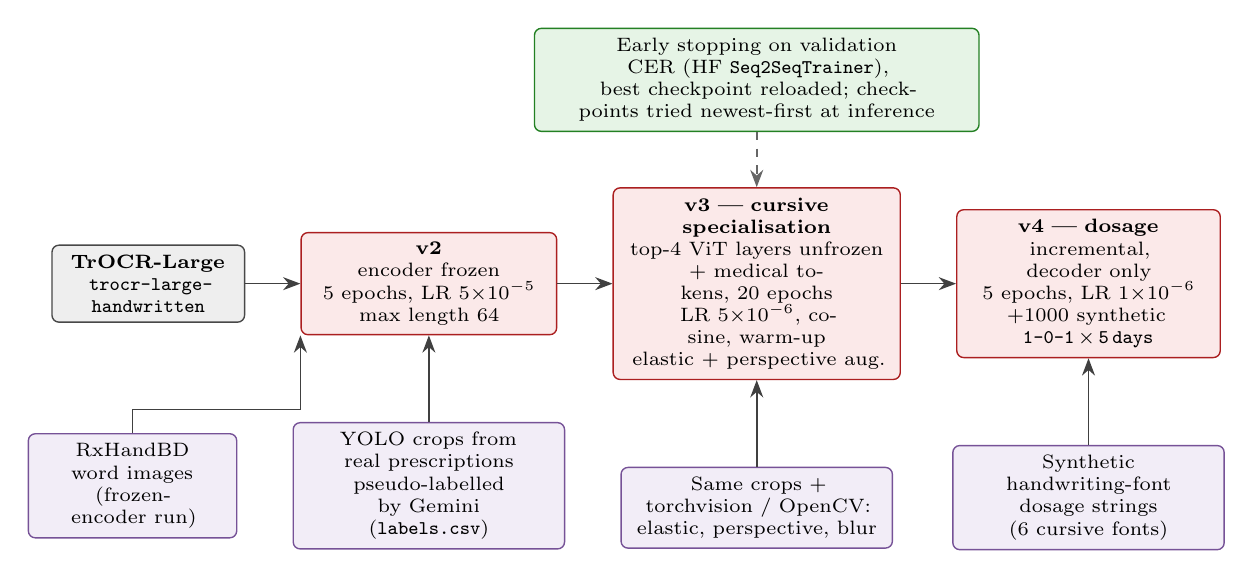
\begin{tikzpicture}[node distance=4mm and 7mm]
  \node[io, text width=2.2cm] (base) {\textbf{TrOCR-Large}\\ \texttt{trocr-large-}\\ \texttt{handwritten}};
  \node[rec, right=of base, text width=3.0cm] (v2) {\textbf{v2}\\ encoder frozen\\ 5 epochs, LR $5{\times}10^{-5}$\\ max length 64};
  \node[rec, right=of v2, text width=3.4cm] (v3) {\textbf{v3 --- cursive specialisation}\\ top-4 ViT layers unfrozen\\ +~medical tokens, 20 epochs\\ LR $5{\times}10^{-6}$, cosine, warm-up\\ elastic + perspective aug.};
  \node[rec, right=of v3, text width=3.1cm] (v4) {\textbf{v4 --- dosage}\\ incremental, decoder only\\ 5 epochs, LR $1{\times}10^{-6}$\\ $+1000$ synthetic \texttt{1-0-1\,$\times$\,5\,days}};
  \draw[arr] (base) -- (v2);
  \draw[arr] (v2) -- (v3);
  \draw[arr] (v3) -- (v4);

  \node[enh, below=11mm of v2, text width=3.2cm] (d1) {YOLO crops from real prescriptions\\ pseudo-labelled by Gemini\\ (\texttt{labels.csv})};
  \node[enh, below=11mm of v3, text width=3.2cm] (d2) {Same crops +\\ torchvision / OpenCV:\\ elastic, perspective, blur};
  \node[enh, below=11mm of v4, text width=3.2cm] (d3) {Synthetic handwriting-font\\ dosage strings\\ (6 cursive fonts)};
  \node[enh, left=of d1, text width=2.4cm] (d0) {RxHandBD\\ word images\\ (frozen-encoder run)};
  \draw[arr] (d1) -- (v2); \draw[arr] (d2) -- (v3); \draw[arr] (d3) -- (v4);
  \draw[arr] (d0.north) |- ++(0,3mm) -| (v2.south west);

  \node[vpost, above=7mm of v3, text width=5.4cm] (cer) {Early stopping on validation CER (HF \texttt{Seq2SeqTrainer}),\\ best checkpoint reloaded; checkpoints tried newest-first at inference};
  \draw[darr] (cer.south) -- (v3.north);
\end{tikzpicture}
}
\caption{TrOCR training lineage and the data feeding each stage.}
\label{fig:training}
\end{figure*}

% =====================================================================
\section{Implementation}\label{sec:impl}
The code base is a single installable Python package, \texttt{mediscript}, organised by pipeline stage (\texttt{detection, preprocessing, recognition, postprocessing, parsing, llm, evaluation, data\_gen, training}). Heavy models are cached across requests, secrets are read from the environment, and all paths derive from one configuration module. A FastAPI service exposes \texttt{POST /analyze} and a static HTML front end (drag-and-drop upload, structured result cards) calls it; a Dockerfile and a command-line entry point are provided. Gemini calls are optional: without a key the system degrades to the local TrOCR route, and LLM stages are skipped. Table~\ref{tab:stack} lists the main components.

\begin{table}[t]
\centering
\caption{Software components.}
\label{tab:stack}
\small
\begin{tabular}{ll}
\toprule
\textbf{Function} & \textbf{Component} \\
\midrule
Line detection & Ultralytics YOLOv8-nano \\
Page OCR & EasyOCR (CRAFT + CRNN) \\
Handwriting OCR & TrOCR-Large (HF Transformers); Gemini 2.5 Flash \\
Fuzzy matching & scikit-learn TF-IDF; RapidFuzz \\
Image processing & OpenCV, Pillow \\
Serving & FastAPI, Uvicorn, HTML/JS \\
Training & PyTorch, HF \texttt{Seq2SeqTrainer}, Colab/Kaggle T4 \\
\bottomrule
\end{tabular}
\end{table}

% =====================================================================
\section{Results and Analysis}\label{sec:results}
We report what was measured and, equally explicitly, what was not. Metrics for recognition are CER and word error rate
\begin{equation}
\mathrm{CER}=\frac{d_{\mathrm{Lev}}(\hat t,t)}{|t|},\qquad
\mathrm{WER}=\frac{d_{\mathrm{Lev}}(\hat{\mathbf w},\mathbf w)}{|\mathbf w|},
\end{equation}
with $d_{\mathrm{Lev}}$ the Levenshtein distance at character and word level; the released \texttt{evaluation} module also reports exact-match accuracy.

\subsection{Field localisation}
Table~\ref{tab:yolo} and Fig.~\ref{fig:yolores} summarise the detector on the held-out portion of D2.

\begin{table}[t]
\centering
\caption{Handwritten-line detection (YOLOv8-nano, single class, 50 epochs).}
\label{tab:yolo}
\begin{tabular}{lr}
\toprule
\textbf{Metric} & \textbf{Value} \\
\midrule
mAP50 & 86.1\% \\
mAP50--95 & 46.2\% \\
Precision & 81.9\% \\
Recall & 80.6\% \\
Training time (Tesla T4) & $\sim$4 min (0.067 GPU-h) \\
Checkpoint size & 6.2\,MB \\
Inference (Tesla T4, per image) & 2.5\,ms \\
\bottomrule
\end{tabular}
\end{table}

\begin{figure}[t]
\centering
\resizebox{0.85\columnwidth}{!}{% Figure: field-localisation metrics (medicine-line detector, 50 epochs, Tesla T4).
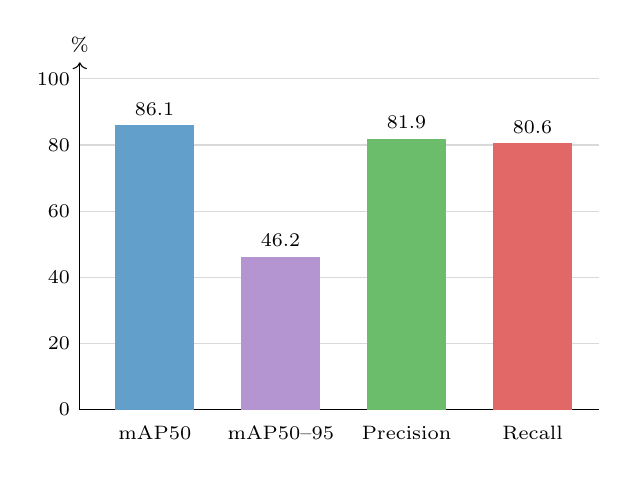
\begin{tikzpicture}[x=1cm,y=0.042cm, font=\scriptsize]
  \draw[->] (0,0) -- (0,105) node[above] {\%};
  \foreach \v in {0,20,40,60,80,100} {
    \draw[black!15] (0,\v) -- (6.6,\v);
    \node[left] at (0,\v) {\v};
  }
  \draw (0,0) -- (6.6,0);
  \foreach \x/\v/\n/\c in {0.45/86.1/mAP50/cDet, 2.05/46.2/mAP50--95/cEnh, 3.65/81.9/Precision/cPost, 5.25/80.6/Recall/cRec} {
    \fill[\c!70] (\x,0) rectangle (\x+1,\v);
    \node[above] at (\x+0.5,\v) {\v};
    \node[below, text width=1.5cm, align=center] at (\x+0.5,-2) {\n};
  }
\end{tikzpicture}
}
\caption{Detector metrics from Table~\ref{tab:yolo}.}
\label{fig:yolores}
\end{figure}

The gap between mAP50 (86.1\%) and mAP50--95 (46.2\%) is typical of handwriting regions: boxes are usually placed on the right line but with imprecise extent, because strokes bleed past nominal field boundaries and annotators drew boxes loosely. Recall trails precision, which we attribute to inconsistent annotation of overlapping or omitted lines; better curation rather than longer training is the promising lever. We have not benchmarked CPU-only inference on edge hardware, so the 2.5\,ms figure should not be read as an edge latency.

\subsection{Qualitative end-to-end analysis}
Early integration tests, run with the confidence-gated pipeline and the curated 1{,}142-entry lexicon, produced two instructive failures.

\paragraph{Case A: in-distribution image.} On a held-out image from D2, YOLO localised four medicine lines correctly. The then-untuned TrOCR returned strings such as \texttt{"wrapportingly ."} and \texttt{"pur-todac itself"} at 32.5--53.8\% confidence---not near-misses of drug names. All four fell below the matching threshold, Stage~3 declined to force a correction, and the record's prescription field stayed \emph{empty}. The system therefore failed \emph{safely}, and the fault was isolated to recognition.

\paragraph{Case B: out-of-distribution image.} On a hospital prescription photographed independently of any training data (Fig.~\ref{fig:ood}), the detector again boxed the medicine line, but the decoder returned a fluent, high-confidence name of an unrelated commercial product. This is the hallucination mode predicted by a general-language prior and the principal reason that domain LM rescoring and lexicon verification are mandatory components rather than refinements.

\begin{figure}[t]
\centering
\begin{subfigure}[b]{0.48\columnwidth}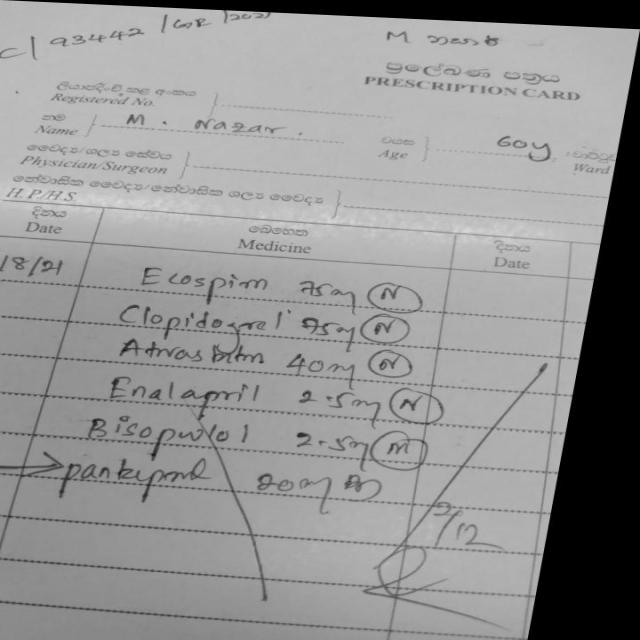
\includegraphics[width=\linewidth]{figures/og_presc.jpg}\caption{Photograph}\end{subfigure}\hfill
\begin{subfigure}[b]{0.48\columnwidth}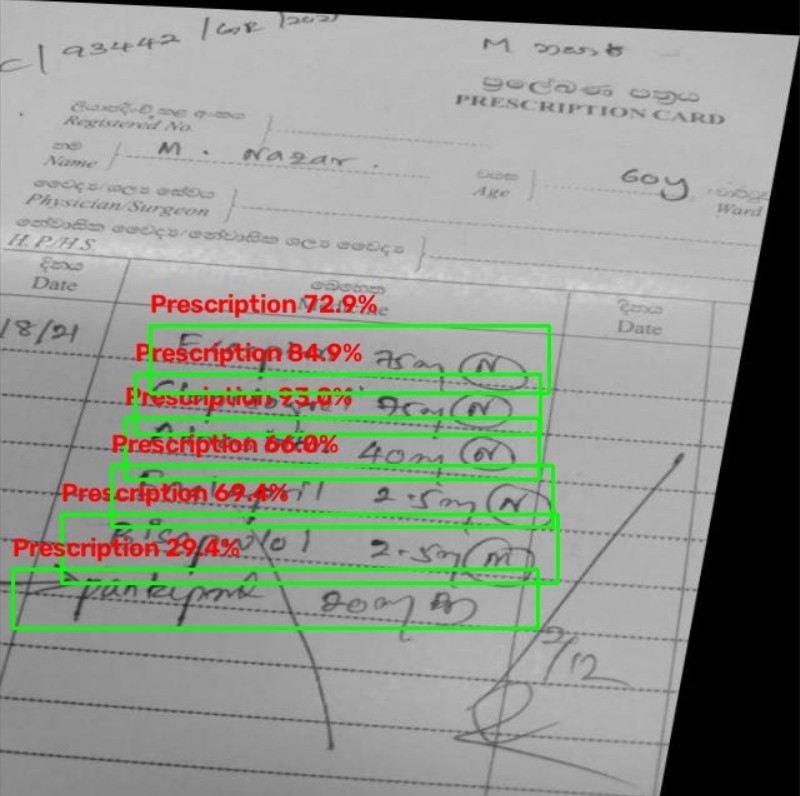
\includegraphics[width=\linewidth]{figures/yolo_presc.jpg}\caption{Stage-1 output}\end{subfigure}
\caption{Out-of-distribution test image (Case B). The detector boxes the handwritten medicine line tightly, localising the fault to recognition.}
\label{fig:ood}
\end{figure}

\subsection{Baseline: end-to-end document transformer}
A pretrained Donut checkpoint fine-tuned only on synthetic digitally rendered prescriptions~\cite{shrivastava2024medocr,kim2022donut}, run on a real photograph, emitted a repeating sequence of full stops irrespective of content---a complete collapse under the synthetic-to-real gap. This supports our decision to keep detection and recognition separate and to train recognisers on real or font-based \emph{handwritten} images.

\subsection{Provenance logging}
An early run seemed to extract the patient's name correctly; inspection showed that a configuration fault had routed the image through a flat-OCR fall-back, and the name was read only because the pad pre-printed ``Name:''. Per-stage provenance logging (console logs report which recogniser handled each crop) was added, and all results in this paper were re-verified against path-level logs.

\subsection{Comparison with the base study}
Table~\ref{tab:baseacc} lists the accuracies reported in the base paper. The paper states different figures in its abstract, results text and conclusion (for instance gender 93.5\% vs.\ 88.6\%, symptoms 90.8\% vs.\ 96.81\%, overall 90.20\%), and they are measured on a proprietary corpus of more than 400{,}000 prescriptions with classification over fixed classes. Our detector metric is a different quantity (localisation) on a public set. \textbf{We therefore make no claim that \sys{} is more accurate than the base system.} What the comparison supports is the design-level argument of Table~\ref{tab:compare}: capabilities that a closed-class classifier cannot provide---open-vocabulary lines, dosage notation, knowledge verification and abstention, layout-free parsing---and a public, re-runnable code and data pipeline.

\begin{table}[t]
\centering
\caption{Accuracies reported by the base paper~\cite{biswas2026novel} (as stated; not reproduced by us and not comparable with Table~\ref{tab:yolo}).}
\label{tab:baseacc}
\small
\begin{tabular}{lcc}
\toprule
\textbf{Attribute} & \textbf{Abstract/figure} & \textbf{Results text} \\
\midrule
Name & 91.2\% & 91.2\% \\
Age & 95.3\% & 94.5\% (1 digit), 89.6\% (multi) \\
Gender & 93.5\% & 88.6\% \\
Symptom & 90.8\% & 96.81\% \\
Medicine & 92.6\% & 95.01\% \\
Printed vs.\ handwritten & --- & 97.3\% (confusion matrix, 1000 patches) \\
\bottomrule
\end{tabular}
\end{table}

\subsection{Component-level summary}
Table~\ref{tab:status} states the evidence behind each component, to prevent over-reading of the results.

\begin{table}[t]
\centering
\caption{Evidence status per component.}
\label{tab:status}
\small
\begin{tabular}{p{2.5cm}p{5.4cm}}
\toprule
\textbf{Component} & \textbf{Evidence} \\
\midrule
YOLO detector & Quantitative (Table~\ref{tab:yolo}) \\
Lexicon gate & Qualitative (Case A; safe failure) \\
Domain LM, trie & Implemented; no ablation reported yet \\
TrOCR v3/v4 & Trained; weights and a real-handwriting CER benchmark not yet released \\
Gemini tier & Implemented; no accuracy measured \\
Spatial parser & Implemented with regression-style fall-backs; no labelled benchmark \\
LLM stage & Implemented; prompt-constrained; not clinically validated \\
\bottomrule
\end{tabular}
\end{table}

% =====================================================================
\section{Discussion}\label{sec:disc}

\subsection{What is new relative to the base study}
\begin{itemize}
  \item \textbf{From classifiers to readers.} Replacing per-attribute CNN--MLP classifiers by a detector plus line-level sequence recognisers removes the closed-vocabulary ceiling and the need to segment glyphs.
  \item \textbf{Verification and abstention.} A large lexicon, a domain LM and, in the gated configuration, a multi-signal confidence rule (Eq.~\ref{eq:conf}) turn recognition errors into empty fields rather than plausible wrong drugs.
  \item \textbf{Dosage and layout.} Synthetic dosage fine-tuning and a spatial parser handle \texttt{1-0-1}-style frequencies and free-form headers, which the base design does not model.
  \item \textbf{Graceful degradation.} Three recognition tiers and optional LLM stages allow the same code to run online (best quality) or offline (local weights only).
  \item \textbf{Reproducibility.} Public data, scripts, a package with accompanying unit tests, an API and a container image replace a proprietary corpus.
\end{itemize}

\subsection{Limitations and threats to validity}
\begin{enumerate}
  \item \textbf{No end-to-end field accuracy.} We have not yet built a transcribed real-prescription benchmark; only localisation is quantified. Case studies are anecdotal.
  \item \textbf{External dependence.} The best reading tier calls a commercial API, subject to latency (the free tier forces $\approx4$\,s delays, giving 20--40\,s per prescription), availability and, critically, patient-data privacy.
  \item \textbf{Data scale and annotation noise.} Detection uses 357 images with loose boxes; D1/D2 include Roboflow augmentations; pseudo-labels from an LLM contain label noise.
  \item \textbf{Scope.} English Latin script; one detector class; the multi-field detector of the original design remains future work. Some test images mix Bengali, which the OCR does not read.
  \item \textbf{Heuristic fragility.} Anchor parsing assumes labels precede values left-to-right; unusual layouts will fail.
  \item \textbf{Gate not in the default path.} The abstention gate was validated in the field-level configuration only; the default page-level path returns uncorrected text, so low-quality readings can appear in the output.
  \item \textbf{Safety.} The system is a research prototype and must not be used for clinical decisions without human verification.
\end{enumerate}

\subsection{Future work}
(i)~Label 200--300 real crops and report CER/WER/exact match for each tier with ablations (no LM, no lexicon, no enhancement); (ii)~expand the detector to the six-field schema and add a text-region classifier for printed vs.\ handwritten text, as in the base paper; (iii)~distil the LLM tier into a local model to remove external dependence; (iv)~calibrate confidences and add a human-review interface; (v)~extend to multilingual scripts and to structured EHR (FHIR) export; (vi)~benchmark CPU and edge latency.

% =====================================================================
\section{Conclusion}\label{sec:conclusion}
\sys{} reframes prescription digitisation as \emph{detect, read, verify}: a 6.2\,MB detector localises handwritten lines (86.1\% mAP50), a tiered recogniser reads them open-vocabulary, a 384{,}604-entry lexicon and a domain language model check the result (with an optional abstention gate), and a spatial parser plus constrained LLM complete the structured record. Compared with a recent CNN--MLP framework trained on a proprietary corpus, the design removes the closed-vocabulary limit, adds knowledge-based verification and an abstention mechanism, and handles dosage notation and free layouts, while remaining reproducible. Its main weakness is the absence of a quantitative end-to-end benchmark on real handwriting; closing that gap is the immediate next step.

\section*{Acknowledgment}
The authors thank the maintainers of the public data sets and open-source libraries used in this work.

\bibliographystyle{IEEEtran}
\bibliography{references}

\end{document}
